\protect\hyperlink{main-nav}{≡} \protect\hyperlink{close-nav}{×}

\hypertarget{section-3.2-the-fundamental-theorem-and-antidifferentiation}{%
\section{Section 3.2: The Fundamental Theorem and
Antidifferentiation}\label{section-3.2-the-fundamental-theorem-and-antidifferentiation}}

\hypertarget{the-fundamental-theorem-of-calculus}{%
\subsection{The Fundamental Theorem of
Calculus}\label{the-fundamental-theorem-of-calculus}}

This section contains the most important and most used theorem of
calculus, the Fundamental Theorem of Calculus. Discovered independently
by Newton and Leibniz in the late 1600s, it establishes the connection
between derivatives and integrals, provides a way of easily calculating
many integrals, and was a key step in the development of modern
mathematics to support the rise of science and technology. Calculus is
one of the most significant intellectual structures in the history of
human thought, and the Fundamental Theorem of Calculus is a most
important brick in that beautiful structure.

To view this video please enable JavaScript, and consider upgrading to a
web browser that \href{http://videojs.com/html5-video-support/}{supports
HTML5 video}

\hypertarget{the-fundamental-theorem-of-calculus-1}{%
\paragraph{The Fundamental Theorem of
Calculus}\label{the-fundamental-theorem-of-calculus-1}}

\textbackslash{}{[} \textbackslash{}int\textbackslash{}limits\_a\^{}b
F'(x) \textbackslash{},dx = F(b) - F(a) \textbackslash{}{]}

This is actually not new for us; we've been using this relationship for
some time; we just haven't written it this way. This says what we've
said before: the definite integral of a rate from
\textbackslash{}(a\textbackslash{}) to
\textbackslash{}(b\textbackslash{}) is the net
\textbackslash{}(y\textbackslash{})-units, the change in
\textbackslash{}(y\textbackslash{}), that accumulate between
\textbackslash{}(t = a\textbackslash{}) and \textbackslash{}(t =
b\textbackslash{}). Here we've just made it plain that that the rate is
a derivative.

Thinking about the relationship this way gives us the key to finding
exact answers for some definite integrals. If the integrand is the
derivative of some \textbackslash{}(F\textbackslash{}), then maybe we
could simply find \textbackslash{}(F\textbackslash{}) and subtract --
that would be easier than approximating with rectangles. Going backwards
through the differentiation process will help us evaluate definite
integrals.

\hypertarget{example-1}{%
\paragraph{Example 1}\label{example-1}}

Find \textbackslash{}(f(x)\textbackslash{}) if \textbackslash{}(f '(x) =
2x\textbackslash{}).

Oooh, I know this one. It's \textbackslash{}( f(x)=x\^{}2+3
\textbackslash{}). Oh, wait, you were thinking something else? Yes, I
guess you're right -- \textbackslash{}( f(x)=x\^{}2 \textbackslash{})
works too. So does \textbackslash{}( f(x)=x\^{}2-\textbackslash{}pi
\textbackslash{}), and \textbackslash{}(
f(x)=x\^{}2+104,\textbackslash{}!589.2 \textbackslash{}). In fact, there
are lots of answers.

In fact, there are infinitely many functions that all have the same
derivative. And that makes sense -- the derivative tells us about the
shape of the function, but it doesn't tell about the location. We could
shift the graph up or down and the shape wouldn't be affected, so the
derivative would be the same.

This leads to one of the trickier definitions -- pay careful attention
to the articles (``the'' versus ``an''), because they're important.

\hypertarget{antiderivatives}{%
\paragraph{Antiderivatives}\label{antiderivatives}}

An \textbf{antiderivative} of a function
\textbackslash{}(f(x)\textbackslash{}) is any function
\textbackslash{}(F(x)\textbackslash{}) where \textbackslash{}(F'(x) =
f(x)\textbackslash{}).

The antiderivative of a function \textbackslash{}(f(x)\textbackslash{})
is a whole family of functions, written \textbackslash{}(F(x) +
C\textbackslash{}), where \textbackslash{}(F'(x) = f(x)\textbackslash{})
and \textbackslash{}(C\textbackslash{}) represents any constant.

The antiderivative is also called the \textbf{indefinite integral}.

\hypertarget{notation-for-the-antiderivative}{%
\subparagraph{Notation for the
Antiderivative}\label{notation-for-the-antiderivative}}

The antiderivative of \textbackslash{}(f\textbackslash{}) is written
\textbackslash{}{[}\textbackslash{}int f(x)
\textbackslash{},dx\textbackslash{}{]}

This notation resembles the definite integral, because the Fundamental
Theorem of Calculus says antiderivatives and definite integrals are
intimately related. But in this notation, there are no limits of
integration.

The \textbackslash{}( \textbackslash{}int \textbackslash{}) symbol is
still called an \textbf{integral sign}; the
\textbackslash{}(dx\textbackslash{}) on the end still must be included;
you can still think of \textbackslash{}( \textbackslash{}int
\textbackslash{}) and \textbackslash{}(dx\textbackslash{}) as left and
right parentheses. The function \textbackslash{}(f\textbackslash{}) is
still called the \textbf{integrand}.

\hypertarget{verb-forms}{%
\subparagraph{Verb Forms}\label{verb-forms}}

We \textbf{antidifferentiate}, or \textbf{integrate}, or \textbf{find
the indefinite integral} of a function. This process is called
\textbf{antidifferentiation} or \textbf{integration}.

There are no small families in the world of antiderivatives: if
\textbackslash{}(f\textbackslash{}) has one antiderivative
\textbackslash{}(F\textbackslash{}), then
\textbackslash{}(f\textbackslash{}) has an infinite number of
antiderivatives and every one of them has the form \textbackslash{}(F(x)
+ C\textbackslash{}).

\hypertarget{example-2}{%
\paragraph{Example 2}\label{example-2}}

Find \textbf{an} antiderivative of \textbackslash{}(2x\textbackslash{}).

We can choose any function we like as long as its derivative is
\textbackslash{}(2x\textbackslash{}), so we can pick, say,
\textbackslash{}( F(x)=x\^{}2-5.2 \textbackslash{}).

\hypertarget{example-3}{%
\paragraph{Example 3}\label{example-3}}

Find \textbf{the} antiderivative of
\textbackslash{}(2x\textbackslash{}).

Now we need to write the entire family of functions whose derivatives
are \textbackslash{}(2x\textbackslash{}). We can use the
\textbackslash{}( \textbackslash{}int \textbackslash{}) notation:
\textbackslash{}{[}\textbackslash{}int 2x\textbackslash{}, dx =
x\^{}2+C.\textbackslash{}{]} (Don't forget the ``\textbackslash{}( +C
\textbackslash{})''!)

\hypertarget{example-4}{%
\paragraph{Example 4}\label{example-4}}

Find \textbackslash{}( \textbackslash{}int e\^{}x\textbackslash{}, dx
\textbackslash{}).

This is likely one you remember: \textbackslash{}( e\^{}x
\textbackslash{}) is its own derivative, so it is also its own
antiderivative. The integral sign tells us that we need to include the
entire family of functions, so we need that
``\textbackslash{}(+C\textbackslash{})'' on the end: \textbackslash{}{[}
\textbackslash{}int e\^{}x\textbackslash{}, dx = e\^{}x+C.
\textbackslash{}{]}

To view this video please enable JavaScript, and consider upgrading to a
web browser that \href{http://videojs.com/html5-video-support/}{supports
HTML5 video}

\hypertarget{antiderivatives-graphically-or-numerically}{%
\subsection{Antiderivatives Graphically or
Numerically}\label{antiderivatives-graphically-or-numerically}}

Another way to think about the Fundamental Theorem of Calculus is to
solve the expression for F(b):

\hypertarget{the-fundamental-theorem-of-calculus-restated}{%
\paragraph{The Fundamental Theorem of Calculus
(restated)}\label{the-fundamental-theorem-of-calculus-restated}}

\textbackslash{}{[} \textbackslash{}int\textbackslash{}limits\_a\^{}b
F'(x) \textbackslash{},dx=F(b) - F(a) \textbackslash{}{]} The definite
integral of a derivative from a to b gives the net change in the
original function.

\textbackslash{}{[}F(b) = F(a) +
\textbackslash{}int\textbackslash{}limits\_a\^{}b F'(x)
\textbackslash{},dx \textbackslash{}{]} The amount we end up is the
amount we start with plus the net change in the function.

This lets us get values for the antiderivative -- as long as we have a
starting point, and we know something about the area.

\hypertarget{example-5}{%
\paragraph{Example 5}\label{example-5}}

Suppose \textbackslash{}(F(t)\textbackslash{}) has the derivative
\textbackslash{}(f(t)\textbackslash{}) shown below, and suppose that we
know \textbackslash{}(F(0) = 5\textbackslash{}). Find values for
\textbackslash{}(F(1),\textbackslash{} F(2),\textbackslash{}
F(3),\textbackslash{}) and \textbackslash{}(F(4)\textbackslash{}).

\begin{figure}
\centering
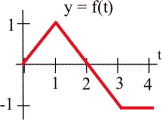
\includegraphics{images/image036.png}
\caption{}
\end{figure}

Using the second way to think about the Fundamental Theorem of Calculus,
\textbackslash{}( F(b) = F(a) +
\textbackslash{}int\textbackslash{}limits\_a\^{}b F'(x)
\textbackslash{},dx \textbackslash{}), we can see that \textbackslash{}(
F(1) = F(0) + \textbackslash{}int\textbackslash{}limits\_0\^{}1 f(x)
\textbackslash{},dx \textbackslash{}). We know the value of
\textbackslash{}(F(0)\textbackslash{}), and we can easily find
\textbackslash{}( \textbackslash{}int\textbackslash{}limits\_0\^{}1 f(x)
\textbackslash{},dx \textbackslash{}) from the graph -- it's just the
area of a triangle. So \textbackslash{}{[}
\textbackslash{}begin\{align*\} F(1) =\&
\textbackslash{}\textbackslash{} =\& 5+0.5
=5.5\textbackslash{}\textbackslash{} F(2) =\& F(0) +
\textbackslash{}int\textbackslash{}limits\_0\^{}2 f(x)
\textbackslash{},dx \textbackslash{}\textbackslash{} =\& 5+1=6
\textbackslash{}end\{align*\} \textbackslash{}{]}

Note that we can start from any place of which we know the value; for
example, now that we know \textbackslash{}(F(2)\textbackslash{}), we can
use that to find \textbackslash{}{[} \textbackslash{}begin\{align*\}
F(3) =\& F(2) + \textbackslash{}int\textbackslash{}limits\_2\^{}3 f(x)
\textbackslash{},dx \textbackslash{}\textbackslash{} =\& 6-0.5=5.5
\textbackslash{}\textbackslash{} F(4) =\& F(3) +
\textbackslash{}int\textbackslash{}limits\_3\^{}4 f(x)
\textbackslash{},dx \textbackslash{}\textbackslash{} =\& 5.5-1=4.5
\textbackslash{}end\{align*\} \textbackslash{}{]}

To view this video please enable JavaScript, and consider upgrading to a
web browser that \href{http://videojs.com/html5-video-support/}{supports
HTML5 video}

Here is a copy of the applet used in this video:

\hypertarget{example-6}{%
\paragraph{Example 6}\label{example-6}}

\textbackslash{}(F'(t) = f(t)\textbackslash{}) is shown below. Where
does \textbackslash{}(F(t)\textbackslash{}) have maximum and minimum
values on the interval {[}0, 4{]}?

\begin{figure}
\centering
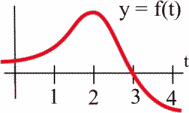
\includegraphics{images/image037.png}
\caption{}
\end{figure}

Since \textbackslash{}( F(b) = F(a) +
\textbackslash{}int\textbackslash{}limits\_a\^{}b F'(x)
\textbackslash{},dx \textbackslash{}), we know that
\textbackslash{}(F\textbackslash{}) is increasing as long as the area
accumulating under \textbackslash{}(F' = f\textbackslash{}) is positive
(until \textbackslash{}(t = 3\textbackslash{})), and then decreases when
the curve dips below the \textbackslash{}(x\textbackslash{})-axis so
that negative area starts accumulating. The area between
\textbackslash{}(t = 3\textbackslash{}) and \textbackslash{}(t =
4\textbackslash{}) is much smaller than the positive area that
accumulates between 0 and 3, so we know that
\textbackslash{}(F(4)\textbackslash{}) must be larger than
\textbackslash{}(F(0)\textbackslash{}). The maximum value is when
\textbackslash{}(t = 3\textbackslash{}); the minimum value is when
\textbackslash{}(t = 0\textbackslash{}).

Note that this is a different way to look at a problem we already knew
how to solve -- in Chapter 2, we would have found critical points of
\textbackslash{}(F\textbackslash{}), where \textbackslash{}(f =
0\textbackslash{}): there's only one, when \textbackslash{}(t =
3\textbackslash{}). \textbackslash{}(f = F'\textbackslash{}) goes from
positive to negative there, so \textbackslash{}(F\textbackslash{}) has a
local max at that point. It's the only critical point, so it must be a
global max. Then we would look at the values of
\textbackslash{}(F\textbackslash{}) at the endpoints to find which was
the global min.

To view this video please enable JavaScript, and consider upgrading to a
web browser that \href{http://videojs.com/html5-video-support/}{supports
HTML5 video}

We can also attempt to sketch a function based on the graph of the
derivative.

\hypertarget{example-7}{%
\paragraph{Example 7}\label{example-7}}

The graph below shows \textbackslash{}(f'(x)\textbackslash{}) -- the
rate of change of \textbackslash{}(f(x)\textbackslash{}). Use it to
sketch a graph of \textbackslash{}(f(x)\textbackslash{}) that satisfies
\textbackslash{}(f(0) = 0\textbackslash{}).

\begin{figure}
\centering
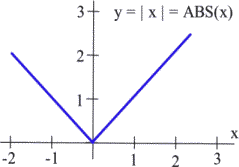
\includegraphics{images/image038.png}
\caption{}
\end{figure}

Recall from the last chapter the relationships between the function
graph and the derivative graph:

\begin{longtable}[]{@{}lllll@{}}
\toprule
\endhead
\textbackslash{}( f(x) \textbackslash{}) & Increasing & Decreasing &
Concave Up & Concave Down\tabularnewline
\textbackslash{}( f'(x) \textbackslash{}) & \textbackslash{}( +
\textbackslash{}) & \textbackslash{}( - \textbackslash{}) & Increasing &
Decreasing\tabularnewline
\bottomrule
\end{longtable}

In the graph shown, we can see the derivative is positive on the
interval (0, 1) and \textbackslash{}((3,
\textbackslash{}infty)\textbackslash{}), so the graph of
\textbackslash{}(f\textbackslash{}) should be increasing on those
intervals. Likewise, \textbackslash{}(f\textbackslash{}) should be
decreasing on the interval (1,3).

In the graph, \textbackslash{}(f'\textbackslash{}) is decreasing on the
interval (0, 2), so \textbackslash{}(f\textbackslash{}) should be
concave down on that interval. Likewise,
\textbackslash{}(f\textbackslash{}) should be concave up on the interval
\textbackslash{}((2, \textbackslash{}infty)\textbackslash{}).

The derivative itself is not enough information to know where the
function \textbackslash{}(f\textbackslash{}) starts, since there are a
family of antiderivatives, but in this case we are given a specific
point at which to start.

To start the sketch, we might note first the shapes we need:

\begin{figure}
\centering
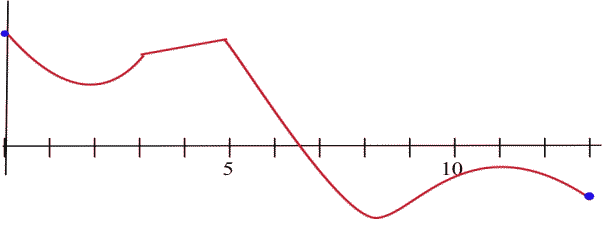
\includegraphics{images/image067.png}
\caption{}
\end{figure}

then sketch the basic shapes:

\begin{figure}
\centering
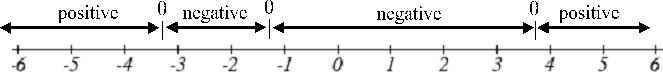
\includegraphics{images/image068.png}
\caption{}
\end{figure}

Now we can attempt to sketch the graph, starting at the point (0, 0).
Notice we are very roughly sketching this, as we don't have much
information to work with. We can tell, though, from the graph that the
area from \textbackslash{}(x = 0\textbackslash{}) to \textbackslash{}(x
= 1\textbackslash{}) is about the same as the area from
\textbackslash{}(x = 1\textbackslash{}) to \textbackslash{}(x =
3\textbackslash{}), so we would expect the net area from
\textbackslash{}(x = 0 \textbackslash{})to \textbackslash{}(x =
3\textbackslash{}) to be close to 0.

\begin{figure}
\centering
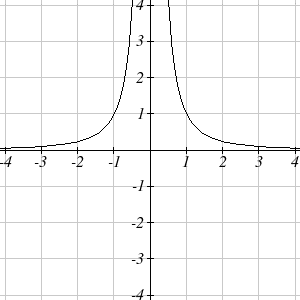
\includegraphics{images/image069.png}
\caption{}
\end{figure}

It turns out this graph isn't horribly bad. Smoothing it out would give
a graph closer to the actual antiderivative graph, shown below.

\begin{figure}
\centering
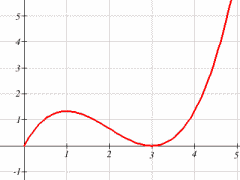
\includegraphics{images/image039.png}
\caption{}
\end{figure}

To view this video please enable JavaScript, and consider upgrading to a
web browser that \href{http://videojs.com/html5-video-support/}{supports
HTML5 video}

\hypertarget{derivative-of-the-integral}{%
\subsection{Derivative of the
Integral}\label{derivative-of-the-integral}}

There is another important connection between the integral and
derivative.

\hypertarget{the-fundamental-theorem-of-calculus-part-2}{%
\paragraph{The Fundamental Theorem of Calculus (part
2)}\label{the-fundamental-theorem-of-calculus-part-2}}

If \textbackslash{}{[}
A(x)=\textbackslash{}int\textbackslash{}limits\_a\^{}x f(t)
\textbackslash{},dt \textbackslash{}{]} then \textbackslash{}{[}
A'(x)=\textbackslash{}frac\{d\}\{dx\}\textbackslash{}int\textbackslash{}limits\_a\^{}x
f(t) \textbackslash{},dt =f(x). \textbackslash{}{]}

I.e., the derivative of the \emph{accumulation function} is the original
function.

To view this video please enable JavaScript, and consider upgrading to a
web browser that \href{http://videojs.com/html5-video-support/}{supports
HTML5 video}

\hypertarget{example-8}{%
\paragraph{Example 8}\label{example-8}}

Let \textbackslash{}(
F(x)=\textbackslash{}int\textbackslash{}limits\_0\^{}x
f(t)\textbackslash{},dt \textbackslash{}), where
\textbackslash{}(f\textbackslash{}) is graphed below. Estimate
\textbackslash{}( F'(3) \textbackslash{}).

\begin{figure}
\centering
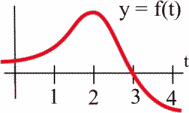
\includegraphics{images/image037.png}
\caption{}
\end{figure}

The function \textbackslash{}(F(x)\textbackslash{}) measures the area
from \textbackslash{}(t = 0\textbackslash{}) to some \textbackslash{}(t
= x\textbackslash{}). To estimate \textbackslash{}( F'(3)
\textbackslash{}), we want to estimate how much the area is increasing
when \textbackslash{}(t = 3\textbackslash{}). Since the value of the
function \textbackslash{}(f(t)\textbackslash{}) is 0 at
\textbackslash{}(t = 3\textbackslash{}), the area will not be increasing
or decreasing, so we can estimate \textbackslash{}( F'(3) = 0
\textbackslash{}).

Directly using the fundamental theorem of calculus part 2,
\textbackslash{}{[} F'(x) =
\textbackslash{}frac\{d\}\{dx\}\textbackslash{}int\textbackslash{}limits\_a\^{}x
f(t) \textbackslash{},dt = f(x) \textbackslash{}{]} so
\textbackslash{}{[} F'(x) = f(3) = 0. \textbackslash{}{]}

\begin{longtable}[]{@{}ll@{}}
\toprule
\endhead
\href{section3-1.php}{← Previous Section} & \href{section3-3.php}{Next
Section →}\tabularnewline
\bottomrule
\end{longtable}
